In this chapter, we address the active target defense differential game where an Attacker missile pursues a Target aircraft. A Defender missile is fired by the Target’s wingman in order to intercept the Attacker before it reaches the aircraft. Thus, a team is formed by the Target and the Defender which
cooperate to maximize the distance between the Target aircraft and the point where the Attacker missile is intercepted by the Defender missile, while the Attacker tries to minimize said distance. The results shown here extend previous work. We consider here the case where the Defender is faster than
the Attacker. The solution to this differential game provides optimal heading angles for the Target and the Defender team to maximize the terminal separation between Target and Attacker and it also provides the optimal heading angle for the Attacker to minimize the said distance.

\begin{figure}[H]
	\centering
	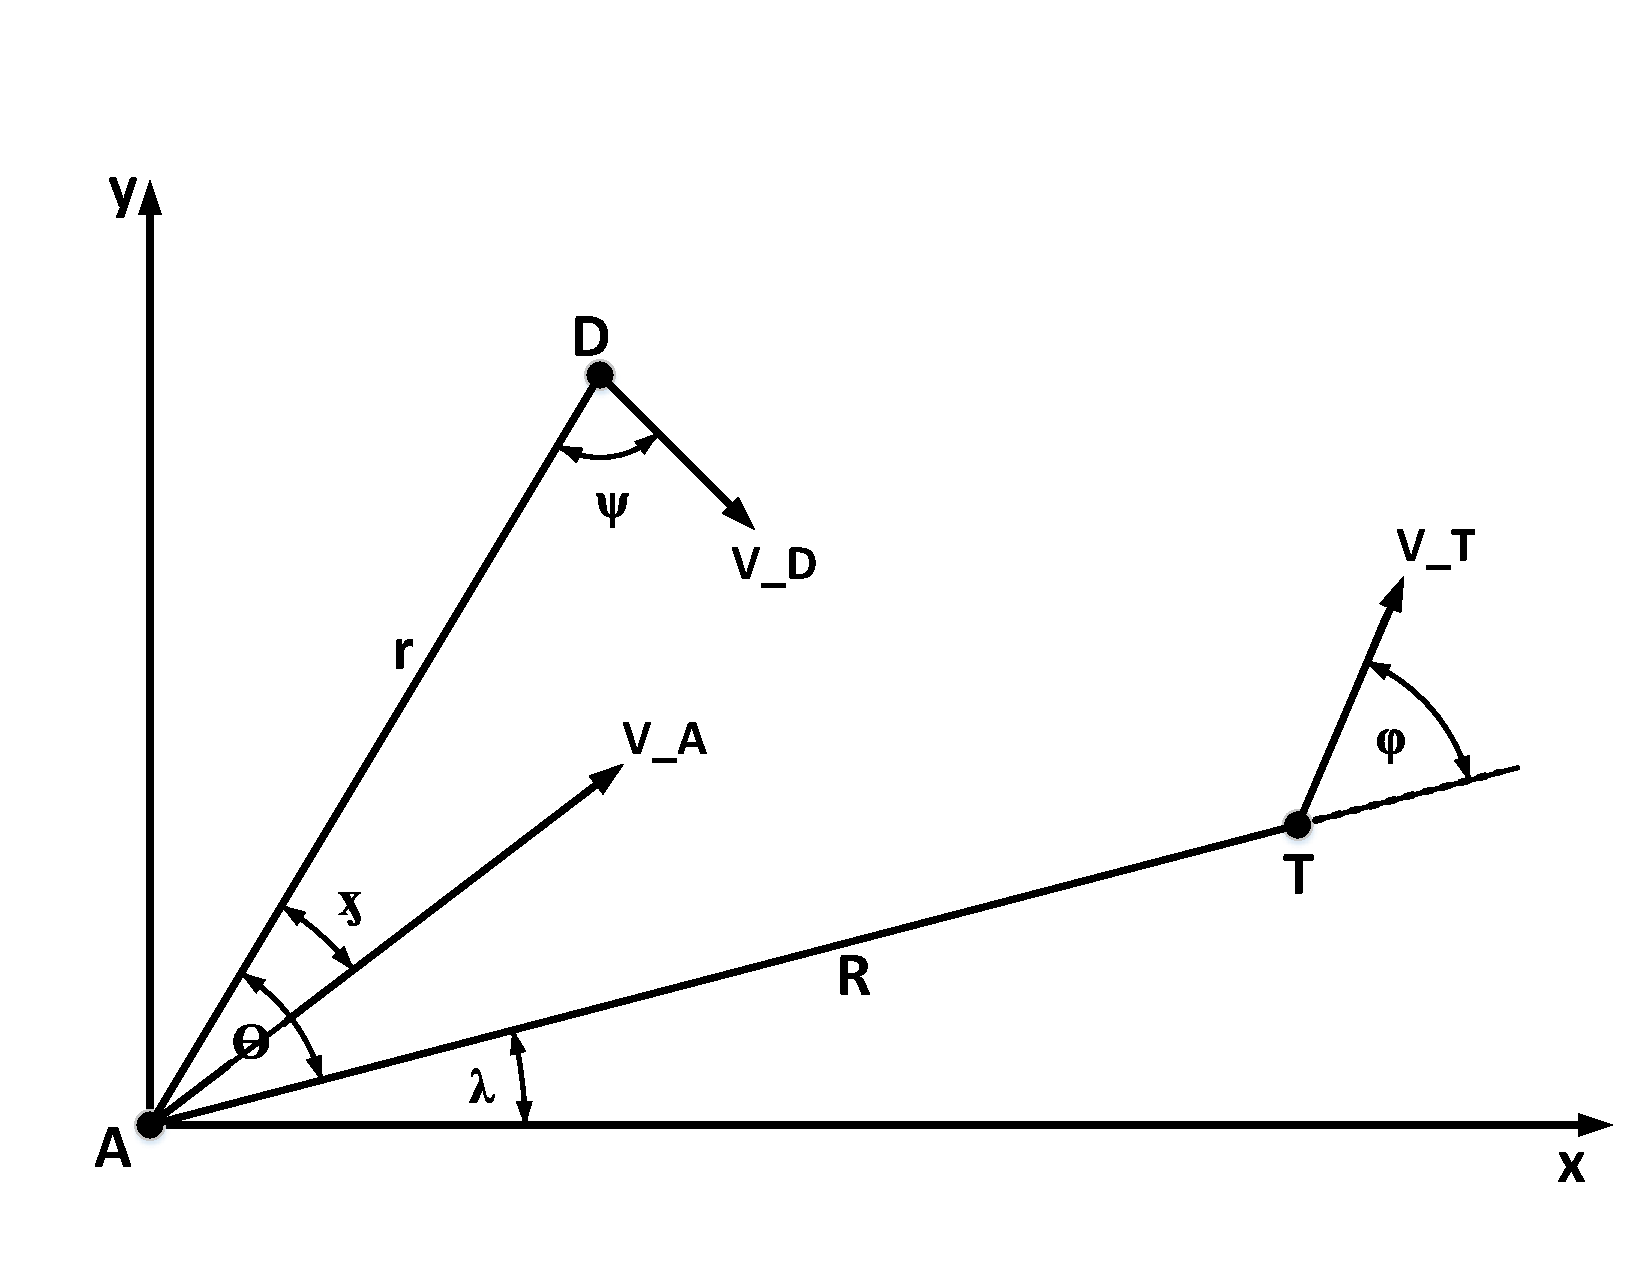
\includegraphics[width=1.0\textwidth]{fig/fig7-1.pdf}
	\caption{State space for the Attacker (A), Target (T), and Defender (D). The origin is arbitrary situated at the Attacker position (A). In polar coordinates with respect to arbitrary coordinates $(x,y)$, the various positions and speeds are}
%		 $A=(0,-)$, $T=(R,\lambda\)$, $D=(r,\lambda+ \theta)$ }
	\label{7.1}
\end{figure}

Figure \ref{7.1} illustrates the state space for the ATD game. The variables $R$ and $r$ are the separations between the Target and Attacker, respectively, and hence denote the radial polar coordinates of the Target and Defender when the origin of coordinates is arbitrarily situated at the position of the Attacker, The speeds of the Attacker, Target and Defender are denoted by $\boldsymbol{V_A}$, $\boldsymbol{V_T}$, $\boldsymbol{V_D}$ with corresponding magnitudes $V_A$, $V_T$ and $V_D$, and polar angles 

\begin{equation}
	Ang\ \boldsymbol{V_A} = \hat{\chi} = \lambda+\theta-\chi
\end{equation}

\begin{equation}
Ang\ \boldsymbol{V_T} = \hat{\phi} = \lambda+\phi
\end{equation}

\begin{equation}
Ang\ \boldsymbol{V_D} = \hat{\psi} = \lambda+\theta-(\pi - \psi)
\end{equation}



The derivatives $\dot{R}$ and $\dot{r}$ can be obtained as differences in radial speeds, while $\dot{\theta}$ can be obtained in terms of the difference in circumferential speeds. The end points of the distance $R$ are moving at a speed $V_T$ at an angle $\phi$ with respect to the radial directions and a speed $V_A$ at an angle $(\theta - \chi)$ with respect to the radial directions. Hence;

\begin{equation}
\begin{split}
\dot{R} &= V_t \cos \phi - V_A \cos(\theta - \chi)\\
&= V_A (\alpha \cos \phi - \cos(\theta - \chi))
\end{split}
\label{Rdot}
\end{equation}

Similarly, we obtain 

\begin{equation}
\begin{split}
\dot{r} &= -V_A \cos \chi - V_D \cos\psi\\
&= V_A (- \cos \chi - \gamma\cos\psi)
\end{split}
\label{rdot}
\end{equation}

In the following, we will deliberately differ from Garcia et.al. []
We will not use \underline{reduced} equations in which $V_A = V_D = 1$.
Our equations will look dimensionally homogeneous to any reader, and we will allow $\gamma = \dfrac{V_D}{V_A}$ to differ from 1.

The circumferential speeds are

\begin{equation*}
\begin{split}
R \dot{\lambda}& = V_T \sin \phi - V_A \sin (\theta - \chi)\\
\dot{\lambda} &= V_A [\dfrac{\alpha}{R} \sin \phi - \dfrac{1}{R} \sin (\theta - \chi)]\\
r (\theta + \lambda)^. &= - V_D \sin \psi + V_A \sin \chi
\end{split}
\end{equation*}  

Hence, one obtains 
\begin{equation}
\dot{\lambda} = V_A [\dfrac{\alpha}{R} \sin \phi - \dfrac{1}{R} \sin (\theta - \chi)]
\label{lambda dot}
\end{equation}

\begin{equation}
\dot{\theta} + \dot{\lambda} = V_A [-\dfrac{\gamma}{r}\sin \psi + \dfrac{1}{r} \sin \chi]
\label{theta+lambda dot}
\end{equation}

Now, subtract (\ref{theta+lambda dot}) minus (\ref{lambda dot}) to obtain

\begin{equation}
\dot{\theta} = V_A [- \dfrac{\alpha}{R} \sin \phi + \dfrac{1}{R} \sin(\theta - \chi) - \dfrac{\gamma}{r} \sin \psi + \dfrac{1}{r}\sin \chi]
\label{theta dot}
\end{equation} 

Equations (\ref{Rdot}), (\ref{rdot}), (\ref{theta dot}) reduce to equations (\ref{lambda dot}) of Garcia et.al [] when we set both $V_A$ and $\gamma=\dfrac{V_D}{V_A}$ equal to 1. 

The system dynamics are given by (\ref{Rdot}), (\ref{rdot}), and (\ref{theta dot}) for $0\lessgtr t \lessgtr t_f$, together with the initial conditions 

\begin{equation*}
	\begin{split}
		R(t_0)&=R_0,\\
		r(t_0)&= r_0,\\
		\theta(t_0)&=\theta_0,
	\end{split}
\end{equation*}

The objective of the Target-Defender team is to maximize
the separation between the Target and the Attacker at the
interception time $R(t_f)$, where the terminal time $t_f$ is free,
such that $r(t_f) = r_c$. The objective of the Attacker is to
minimize the same distance $R(t_f)$. This can be expressed as

\begin{equation*}
max_{\phi,\psi}\ min_\chi\ J= \int_{t_0}^{t_f} \dot{R}\ dt
\end{equation*}

The Hamiltonian is
\begin{equation}
	\begin{split}
	H = & \cos(\theta - \chi) - \alpha \cos \phi \\
	& + [\alpha \cos \phi  - \cos (\theta - \chi)]\ \lambda_R \\
	& - [\cos\chi + \cos\psi]\ \lambda_r \\
	& + [-\frac{\alpha}{R}\sin\phi 
	+\frac{1}{R}\sin(\theta - \chi )
	-\frac{1}{r} \sin \psi
	+\frac{1}{r} \sin \chi]\ \lambda_\theta
	\end{split}
	\label{Hamiltonian}
\end{equation}


\begin{equation*}
	\begin{split}
		H = & -(1-\lambda_R) [\alpha \cos \phi - \cos(\theta - \chi)]\\
		& - [\cos\chi + \beta \cos \psi ]\ \lambda_R \\
		& + [-\frac{\alpha}{R} \sin \phi + \frac{1}{R} \sin (\theta - \chi) - \dfrac{\beta}{r} \sin \psi + \frac{1}{r} \sin \chi ]\ \lambda_\theta 
	\end{split}
\end{equation*}

%============================================================================================
\begin{figure}[ht!]
	\centering
	\newcommand{\pythagwidth}{4cm}
	\newcommand{\pythagheight}{3cm}
	
	\begin{minipage}{.5\textwidth}
		\centering
		\begin{tikzpicture}
			% Define the 3 nodes A, B, C
			\coordinate [label={below right:$A$}] (A) at (0, 0);
			\coordinate [label={above right:$B$}] (B) at (0, \pythagheight);
			\coordinate [label={below left:$C$}] (C) at (-\pythagwidth, 0);	
			% Draw the triangle
			\draw [very thick] (A) -- (C) -- (B) -- cycle;
			% Draw the square angle 
			\newcommand{\ranglesize}{0.3cm}
			\draw (A) rectangle (-\ranglesize,\ranglesize);
			\draw [dashed] (A) -- node [below] {$\lambda_r$} ++ (C);
			\draw [dashed] (A) -- node [right] {$\dfrac{\lambda_\theta}{r}$} ++ (B);
			\draw [dashed] (C) -- node [above,sloped]  {$[(\frac{\lambda_\theta}{r})^2 + \lambda_r^2]^\frac{1}{2}$} (B);
			% fill in the angle
			\filldraw[fill=green!20!white, draw=green!50!black] (C) -- (-3.7,0) arc (0:36.8: 0.3) -- cycle;
			% label of the angle
			\coordinate [label={below left:$\psi^*$}] (angle) at (-2.7, 0.6);
		\end{tikzpicture}
		
		\caption{Defender}
		
	%	\label{optimal heading angles}
	\end{minipage}
	
		\begin{minipage}{.5\textwidth}
			\centering
			\begin{tikzpicture}
			% Define the 3 nodes A, B, C
			\coordinate [label={below right:$A$}] (A) at (0, 0);
			\coordinate [label={above right:$B$}] (B) at (0, \pythagheight);
			\coordinate [label={below left:$C$}] (C) at (-\pythagwidth, 0);	
			% Draw the triangle
			\draw [very thick] (A) -- (C) -- (B) -- cycle;
			% Draw the square angle 
			\newcommand{\ranglesize}{0.3cm}
			\draw (A) rectangle (-\ranglesize,\ranglesize);
			\draw [dashed] (A) -- node [below] {$1-\lambda_r$} ++ (C);
			\draw [dashed] (A) -- node [right] {$\dfrac{\lambda_\theta}{R}$} ++ (B);
			\draw [dashed] (C) -- node [above,sloped]  {$[(\frac{\lambda_\theta}{R})^2 + (1-\lambda_r)^2]^\frac{1}{2}$} (B);
			% fill in the angle
			\filldraw[fill=green!20!white, draw=green!50!black] (C) -- (-3.7,0) arc (0:36.8: 0.3) -- cycle;
			% label of the angle
			\coordinate [label={below left:$\phi^*$}] (angle) at (-2.7, 0.6);
			\end{tikzpicture}
			
			\caption{Target}
			
			%\label{optimal heading angles}
		\end{minipage}
		
			\begin{minipage}{.5\textwidth}
				\centering
				\begin{tikzpicture}
				% Define the 3 nodes A, B, C
				\coordinate [label={below right:$A$}] (A) at (0, 0);
				\coordinate [label={above right:$B$}] (B) at (0, \pythagheight);
				\coordinate [label={below left:$C$}] (C) at (-\pythagwidth, 0);	
				% Draw the triangle
				\draw [very thick] (A) -- (C) -- (B) -- cycle;
				% Draw the square angle 
				\newcommand{\ranglesize}{0.3cm}
				\draw (A) rectangle (-\ranglesize,\ranglesize);
				\draw [dashed] (A) -- node [below] {$\chi_c$} ++ (C);
				\draw [dashed] (A) -- node [right] {$\chi_s$} ++ (B);
				\draw [dashed] (C) -- node [above,sloped]  {$(\chi_s^2 +\chi_c^2)^\frac{1}{2} $} (B);
				% fill in the angle
				\filldraw[fill=green!20!white, draw=green!50!black] (C) -- (-3.7,0) arc (0:36.8: 0.3) -- cycle;
				% label of the angle
				\coordinate [label={below left:$\chi^*$}] (angle) at (-2.7, 0.6);
				\end{tikzpicture}
				
				\caption{Attacker}
				
			%	\label{optimal heading angles}
			\end{minipage}
			
	\caption{Right-angled triangles that define the optimal headings $\psi^*$, $\phi^*$ and $\chi^*$ for the Defender, Target, and Attacker, respectively}
	
	\label{optimal heading angles}
	
\end{figure}




%====================================================================================


We now find the optimal heading angles $\psi^*$, $\phi^*$ and $\chi^*$. Since these angles are known to be positive or negative angles (ranging from $\frac{-\pi}{2}$ to $\frac{\pi}{2}$), it suffices to determine the tangent $\tan a$ of each angle $a$ and then determine the cosine and sine from

\begin{equation}
	\cos a = [1+ \tan^2 a ]^{\frac{-1}{2}}
	\label{cos a}
\end{equation}

\begin{equation}
\sin a =\tan a [1+ \tan^2 a ]^{\frac{-1}{2}}
\label{sin a}
\end{equation}

We obtain $\psi^*$ by partially differentiating the Hamiltonian (\ref{Hamiltonian}) w.r.t. $\psi$ and equating the derivative $\frac{\partial H}{\partial \psi}$ to zero, namely 

\begin{equation}
	\frac{\partial H}{\partial \psi} = \beta \lambda_r \sin \psi - \frac{\beta}{r} \lambda_\theta \cos \psi = 0 
\label{PD H wrt psi}
\end{equation}

Hence the optimal heading $\psi^*$ is given by:

\begin{equation}
	\tan \psi^* = \dfrac{\lambda_\theta / r}{\lambda_r}
\label{tan psi}
 \end{equation}
 
 Figure \ref{optimal heading angles} shows that $\psi^*$ is a (positive or negative) acute angle in a right-angled triangle with an opposite side equal to ($\lambda_\theta / r$), an adjacent side equal to $\lambda_r$ and a hypotenuse equal to $[(\frac{\lambda_\theta}{r})^2 + \lambda_r^2]^\frac{1}{2}$. Using Fig.\ref{optimal heading angles} or relations (\ref{cos a}) and (\ref{sin a}) one obtains 
 
\begin{equation}
 	\cos \psi^* = \lambda_r [(\frac{\lambda_\theta}{r})^2 + \lambda_r^2]^\frac{-1}{2} 
 	= \dfrac{r \lambda_r}{\sqrt{\lambda_\theta ^2 + r^2 \lambda_r ^2}}
\label{cos psi}
\end{equation}

\begin{equation}
\sin \psi^* = (\frac{\lambda_\theta}{r}) [(\frac{\lambda_\theta}{r})^2 + \lambda_r^2]^\frac{-1}{2} 
= \dfrac{\lambda_\theta}{\sqrt{\lambda_\theta ^2 + r^2 \lambda_r ^2}}
\label{sin psi}
\end{equation}

We further compute the second partial derivative of the Hamiltonian w.r.t. $\psi$, that is 

\begin{equation}
\begin{split}
\frac{\partial^2 H}{\partial \psi^2}& = \beta \lambda_r \cos \psi + \beta \frac{\lambda_\theta }{r} \sin \psi \\
&= [\beta r \lambda^2 _ r + \beta \frac{\lambda^2 _ \theta}{r}][\lambda^2_\theta + r^2 \lambda^2_r]^\frac{-1}{2} > 0
\end{split}
\end{equation}

The fact that $\frac{\partial^2 H}{\partial \psi^2}>0$ means that the extremum obtained by (\ref{PD H wrt psi}) is a minimum, i.e., the optimal value $\psi^*$ minimizes the cost ($-J$).

We now obtain $\phi^*$ by partially differentiating Hamiltonian (\ref{Hamiltonian}) w.r.t. $\phi$ and equating the partial derivative $\frac{\partial H}{\partial \phi}$ to zero, namely 

\begin{equation} 
	\frac{\partial H}{\partial \phi} = \alpha (1-\lambda_R) \sin \phi - \frac{\alpha}{R} \lambda_\theta \cos \phi =0 
\label{PD H wrt phi}
\end{equation} 

Hence the optimal heading $\phi^*$ is given by 

\begin{equation}
	\tan \phi^* = \dfrac{(\lambda_\theta/R)}{1- \lambda_R}
\label{tan phi}
\end{equation}

Figure \ref{optimal heading angles} shows that $\phi^*$ is a positive or negative acute angle in a right-angled triangle with an opposing side of length ($\lambda_\theta/R$), an adjacent side of length ($1- \lambda_R$), and a hypotenuse of length $[(\lambda_\theta/R)^2+(1-\lambda_R)^2]^\frac{1}{2}$.

Using Fig.\ref{optimal heading angles} or relations (\ref{cos a}) and (\ref{sin a}), we obtain


\begin{equation}
	\cos \phi^* = (1-\lambda_R)[(\lambda_\theta/R)^2+(1-\lambda_R)^2]^\frac{-1}{2} 
	= \dfrac{R (1- \lambda_R)}{\sqrt{\lambda^2 _\theta + R^2 (1-\lambda_R)^2}}
\label{cos phi}
\end{equation}


\begin{equation}
\sin \phi^* = (\lambda_\theta /R)[(\lambda_\theta/R)^2+(1-\lambda_R)^2]^\frac{-1}{2} 
= \dfrac{\lambda_\theta}{\sqrt{\lambda^2 _\theta + R^2 (1-\lambda_R)^2}}
\label{sin phi}
\end{equation}

The second partial derivative of the Hamiltonian w.r.t. $\phi$ is given by 

\begin{equation}
\begin{split}
\frac{\partial^2 H}{\partial \phi^2}& = \alpha(1- \lambda_R)  \cos \phi +  \frac{\alpha }{R}\lambda_\theta \sin \phi \\
&= [\alpha R (1-\lambda_R)^2 +\frac{\alpha}{R} \lambda^2 _ \theta  ][\lambda^2_\theta + R^2 (1-\lambda_R)^2]^\frac{-1}{2} > 0
\end{split}
\end{equation}

The fact that $\frac{\partial^2 H}{\partial \phi^2}>0$ means that the extrema obtained by (\ref{PD H wrt phi}) is minimum, i.e., the optimal heading $\phi^*$ minimizes the cost $(-J)$.

Finally, we obtain the optimal heading $\chi^*$ by partially differentiating the Hamiltonian (\ref{Hamiltonian}) w.r.t. $\chi$ and equating the partial derivative $\frac{\partial H}{\partial \chi}$ to zero, namely

\begin{equation}
	\frac{\partial H}{\partial \chi} = (1-\lambda_R) \sin(\theta - \chi) + \lambda_r \sin \chi 
	- \frac{\lambda_\theta}{R} \cos (\theta - \chi) + \frac{\lambda_\theta}{r} \cos \chi = 0
\label{PD H wrt chi}
\end{equation}

Using the trigonometric expansions: 

\begin{equation}
	\sin(\theta - \chi) = \sin \theta\ \cos\chi - \cos \theta\ \sin\chi 
\end{equation}

\begin{equation}
\cos(\theta - \chi) = \cos \theta\ \cos\chi + \sin \theta\ \sin\chi 
\end{equation}

We can rewrite (\ref{PD H wrt chi}) in the form 

\begin{equation}
		\frac{\partial H}{\partial \chi} = \chi_s \cos\chi - \chi_c \sin \chi =0
\label{PD H wrt chi 2}
\end{equation}

where 

\begin{equation}
	\chi_s = (1-\lambda_R) \sin\theta - \frac{\lambda_\theta}{R} \cos\theta + \frac{\lambda_\theta}{r}
\end{equation}

\begin{equation}
	\chi_c = (1-\lambda_R) \cos \theta + \frac{\lambda_\theta}{R} \sin \theta - \lambda_r
\end{equation}


The optimal heading $\chi^*$ is obtained from (\ref{PD H wrt chi 2}) as  

\begin{equation}
	\tan \chi^* = \dfrac{\chi_s}{\chi_c}
\label{tan chi}
\end{equation}

Figure \ref{optimal heading angles} shows that $\chi^*$ is a positive or negative acute angle in a right-angled triangle with an opposing leg of length $\chi_s$, an adjacent leg of length $\chi_c$, and a hypotenuse of length $[\chi^2_s+ \chi^2_c]^\frac{1}{2}$. Using Fig. \ref{optimal heading angles} or relations (\ref{cos a}) and (\ref{sin a}), we obtain 


\begin{equation}
	\cos \chi^* = \chi_c\ [\chi^2_s + \chi^2_c]^\frac{-1}{2}
	= \dfrac{\chi_c}{\sqrt{\chi^2_s + \chi^2_c}} 
\end{equation}

\begin{equation}
\sin \chi^* = \chi_s\ [\chi^2_s + \chi^2_c]^\frac{-1}{2}
= \dfrac{\chi_s}{\sqrt{\chi^2_s + \chi^2_c}} 
\end{equation}


The second derivative of the Hamiltonian w.r.t. $\chi$ is obtained from (\ref{PD H wrt chi 2}) as 

\begin{equation}
\begin{split}
\frac{\partial^2 H}{\partial \chi^2}& = -\chi_s  \sin \chi - \chi_c \cos \chi \\
&=-[\chi^2_s + \chi^2_c] (\chi^2_s + \chi^2_c)^\frac{-1}{2} \\
&=- (\chi^2_s + \chi^2_c)^\frac{1}{2}> 0
\end{split}
\label{2PD H wrt chi}
\end{equation}

Equation (\ref{2PD H wrt chi}) demonstrates definitely that $\frac{\partial^2 H}{\partial \chi^2}$ is negative. The corresponding claim via Eq.(28) of Garcia et. al. [] is not complete. The fact that $\frac{\partial^2 H}{\partial \chi^2}<0$ means that the extremum obtained via (\ref{PD H wrt chi 2}) is a maximum, i.e., the optimal heading $\chi^*$ maximizes the cost $(-J)$.

In passing, we note that (\ref{PD H wrt chi}) can be simplified via (\ref{cos psi}), (\ref{sin psi}), (\ref{cos phi}) and (\ref{sin phi}) to give:

\begin{equation}
\begin{split}
	\frac{\partial H}{\partial \chi} &= [(\frac{\lambda_\theta}{R})^2+(1-\lambda_R)^2]^\frac{1}{2} [\cos \phi \sin (\theta-\chi) - \sin \phi \cos (\theta - \chi )]
	+[(\frac{\lambda_\theta}{r})^2 + \lambda^2_r]^\frac{1}{2} [\cos \psi \sin \chi + \sin \psi \cos \chi]\\
	&=[(\frac{\lambda_\theta}{R})^2+(1-\lambda_R)^2]^\frac{1}{2} \sin (\theta - \chi - \phi)   + [(\frac{\lambda_\theta}{r})^2 + \lambda^2_r]^\frac{1}{2} \sin (\chi + \psi)  =0
\end{split}
\end{equation}

The expressions for the optimal heading angles (\ref{tan psi}), (\ref{tan phi}), and (\ref{tan chi}) are to be used in the numerical solution of the Two-Point Boundary Value Problem (TPBVP). That solution is found by substituting the optimal headings into the state equations (), and the co-state rquations ()  with the terminal conditions (). 